\documentclass [a4paper, 12pt] {article}
\usepackage [T1] {fontenc}
\usepackage [utf8] {inputenc}
\usepackage [slovene] {babel}
\usepackage {url}
\usepackage{graphicx}

\title {Vislice}
\author {Matic Oskar Hajšen, Ines Meršak}
\date {\today}

\begin {document}

\maketitle
\tableofcontents

\newpage

\section {Opis projekta}
Cilj najinega projekta je izdelati igrico vislice, pri čemer program izbere naključno besedo za ugibanje s spletnega Slovarja slovenskega knjižnega jezika, ki se nahaja na povezavi \url{http://bos.zrc-sazu.si/sskj.html}.
\subsection {Zahteve projekta}
\begin {itemize}
\item Izbrati naključno besedo iz spletnega slovarja.
\item Podatkovna struktura, ki bo sledila napredku uporabnika -- kolikšen del besede je že uganjen in koliko poskusov je še ostalo.
\item Grafični vmesnik, ki bo prikazoval napredek uporabnika, in vodil statistiko.
\item  Pridobitev definicije izbrane besede po koncu igre, vkolikor uporabnik to želi.
\end {itemize}

\section {Opis spletnega podatkovnega vira}
Spletni SSKJ vsebuje iskalnik besed, v katerega se da vpisati več parametrov, da je iskanje še bolj omejeno. Lahko se določi dolžina besed, preveri, ali opis besede vsebuje določen kvalifikator, in kako natančno mora beseda ustrezati iskanemu geslu. URL naslov strani, na katerih se prikažejo rezultati iskanja, so odvisni od vnešenega gesla iskanja. Na eni strani je do 25 besed, urejenih po abecednem redu. Vsaka beseda je oštevilčena in številka prve prikazane besede je določena v URL naslovu. Stran uporablja unicode za zapis šumnikov in naglašenih črk.
\subsection {Opis načina pridobivanja podatkov}
Za pridobivanje podatkov s spletnega vira sta uporabljena modula \textbf {re} in \textbf {requests} in iskalnik na strani. Beseda, ki se jo v igri uganjuje, je izbrana naključna beseda iz seznama vseh besed v SSKJ, ki je rezultat iskanja z geslom "*". Definicije posameznih besed, ki se lahko prikažejo na koncu igre, so najdene z geslom "ge=beseda", ki vrne le to besedo.


\section {Opis podatkovnega modela}
Projekt je razdeljen na:
\begin {enumerate}
\item pridobivanje besede in definicije s spletnega slovarja in obdelava teh podatkov,
\item programiranje ustreznega podatkovnega tipa za hranjenje besede, definicije, in drugih uporabnih podatkov o igri,
\item programiranje grafičnega vmesnika.
\end {enumerate}

\subsection {Metode za branje in obdelavo podatkov}
Za igro je najbolj potrebna funkcija \textbf {random\_beseda}, ki pa temelji na vrsti pomožnih funkcij.
\begin {itemize}
\item \textbf {je\_slovensko}: Preveri, ali je beseda ustrezna. To pomeni, da ne vsebuje črk, ki niso iz slovenske abecede, in, da ne vsebuje presledkov ali vezajev.
\item \textbf {naglasi}: Zamenja unicode zapis šumnikov in naglašenih črk z ustrezno črko.
\item \textbf {naslov}: Iz vnešenega gesla ustvari URL naslov, ki ustreza strani rezultatov iskanja.
\item \textbf {stevilo\_besed}: Vrne število zadetkov iskanja.
\item \textbf {najdi\_sskj}: Išče besede, glede na podane omejitve, in v ta namen uporablja zgoraj opisane funkcije. Ločena sta dva različna primera:
\begin {itemize}
\item Iskano geslo omejimo z "ge=": to pomeni, da išče le besede, ki geslo vsebujejo in se ne pojavlja le v njihovem opisu. V tem primeru funkcija poišče vse besede na strani, nato pa gre na naslednjo tako, da poveča številko v URL naslovu za 25.
\item Če vpišemo le niz sam, se niz v rezultatih obarva z rdečo. Na ta način najde tudi besede, ki imajo niz samo v opisu. Funkcija tako išče besede, ki so obarvane rdeče, in se ustavi, ko pride do besede, ki je povsem črna.
\end {itemize}
\item \textbf {random\_beseda}: Uporabi \textbf {najdi\_sskj}, da poišče naključno besedo. Funkcija si izbere naključno število in ga nato ustavi v URL naslov iskanja z "*", ki vrne vse besede. Potem izbere prvo ustrezno besedo, saj je mogoče, da je izbrana neustrezna.
\item \textbf {definicija}: Poišče definicijo v opisu iskane besede, ki so običajno napisane poševno.
\end {itemize} 
Obstaja tudi dve funkciji, ki nista uporabljeni v končnem izdelku. Tak način iskanja naključnh besed je bil prepočasen.
\begin {itemize}
\item \textbf {random\_crke}: Izbere tri naključne črke in iz njih ustvari niz. Nastaviti se da težavnost, ki določi, ali niz vsebuje samoglasnike ali ne.
\item \textbf {random\_besede}: Po SSKJ išče besede, ki vsebujejo niz, ustavarjen z zgornjo funkcijo. Če ni takšnih besed, uporabi nov niz in tako ponavlja, dokler ne najde besede. Takšno iskanje traja predolgo, zato se uporablja nova funkcija \textbf {random\_beseda}.
\end {itemize}

\subsection {Razred Beseda}
Razred Beseda vsebuje atribute beseda, definicija, neznano, znano, preostali\_poskusi in ugibano ter metode velike, za\_gui, ugibaj in reseno.
\subsubsection {Atributi}
\begin {itemize}
\item \textbf {beseda}: Vsebuje izbrano besedo za vislice.
\item \textbf {definicija}: Vsebuje definicijo besede; ob klicu konstruktorja je vrednost definicije privzeto None.
\item \textbf {neznano}: Vsebuje črke besede, ki še niso bile ugibane; na začetku je to kar cela beseda. 
\item \textbf {znano}: Vsebuje niz, ki predstavlja trenutno znane dele besede. Na mestu črk, ki so neznane, stoji podčrtaj. Na začetku je ta niz sestavljen iz toliko podčrtajev, kolikor je dolga beseda.
\item \textbf {preostali\_poskusi}: Števec, ki beleži število preostalih poskusov uporabnika; na začetku je vrednost tega atributa nastavljena na 11. 
\item \textbf {ugibano}: Niz, ki beleži, katere črke je uporabnik že ugibal; na začetku je niz prazen.
\end {itemize}
\subsubsection {Metode}
\begin {itemize}
\item \textbf {velike}: Vrne izbrano besedo, torej atribut beseda, napisano z velikimi črkami.
\item \textbf {za\_gui}: Do sedaj znane dele besed, torej atribut znano, pripravi za prikaz v grafičnem vmesniku, tako da med črke oziroma podčrtaje doda poljubno število presledkov, in pripravljen niz vrne. Če je igre konec, potem vrne že povsem odkrito besedo, brez podčrtajev. 
\item \textbf{ugibaj}: Sprejme ugiban znak (deluje tudi za nize) uporabnika. Preveri znak: če ta ni v slovenski abecedi, vrne napako; če je znak med že ugibanim znaki, ne naredi ničesar; če je znak del besede, metoda posodobi atribute znano, neznano in ugibano; če znak ni del besede, pa posodobi atribute ugibano in preostali\_poskusi. Če se je atribut znano spremenil, potem metoda vrne ta atribut, sicer pa ne vrne ničesar. 
\item \textbf{reseno}: Preveri, ali je uporabnik že uganil iskano besedo.
\end {itemize}

\section {Uporabniški vmesnik}
\begin {figure} [h]
\centering
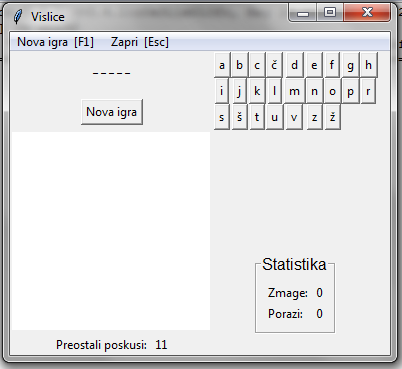
\includegraphics [height=190pt] {slike/za_porocilo_gui.png}
\caption {Grafični vmesnik na začetku nove igre.}
\end {figure}
\noindent Grafični vmesnik je sestavljen iz preprostega menija in glavnega okna.  Glavno okno je razdeljeno na štiri razdelke. \\
Levo zgoraj se nahaja Label z do zdaj uganjeno besedo, gumb za začetek nove igre, ob koncu igre pa se tam pojavi tudi gumb za pridobitev definicije in Label z definicijo. \\
Levo spodaj se nahaja platno s spreminjajočo se sliko, ki uporabniku pove, koliko je 'obešen', pod platnom pa se nahaja še števec preostalih poskusov.  \\
Desno zgoraj se nahaja tipkovnica, sestavljena iz gumbov, s pomočjo katerih lahko uporabnik vnaša znake. \\
Desno spodaj pa je okvirček s statistiko, ki beleži uporabnikove zmage in poraze za trenutno sejo. 
\subsection {Navodila za uporabo}
Ko uporabnik zažene datoteko gui.py, lahko takoj prične z igro. Znake lahko vnaša s pomočjo gumbov, ki se nahajajo desno zgoraj v glavnem oknu programa, ali s pomočjo tipkovnice. Pri tem se za vsak pravilno uganjen znak posodobi Label z do zdaj uganjeno besedo , za vsak napačen znak pa se posodobi slika, števec preostalih poskusov pa se zmanjša za 1. Ob koncu igre se ne glede na zmago ali poraz uporabnika odkrije celotna beseda, prav tako pa se levo zgoraj pojavi gumb 'Definicija', ki poskrbi za prikaz definicije ob kliku nanj. Prav tako se ob koncu igre zabeleži zmaga ali poraz v okvirčku 'Statistika' in, vkolikor je uporabnik zgubil, se prikaže slabo narisana slika obešenega človečka. \\
Uporabnik lahko novo igro prične s pomočjo gumba 'Nova igra', izbire 'Nova igra' v meniju ali gumba F1. \\
Uporabnik lahko zapre program s klikom na rdeč križec v desnem zgornjem kotu okna, izbiro 'Izhod' v meniju ali s pritiskom na gumb Esc.
\begin {figure} [h]
\centering
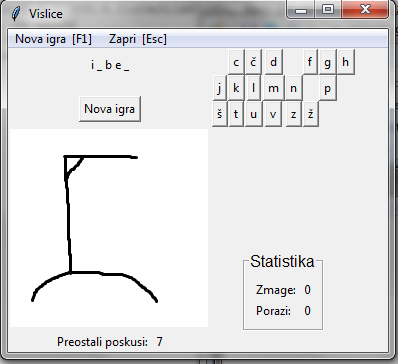
\includegraphics [width=125pt] {slike/za_porocilo_gui_progress.png}
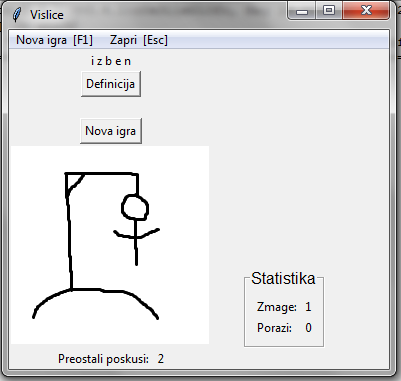
\includegraphics [width=125pt] {slike/za_porocilo_gui_zmaga.png}
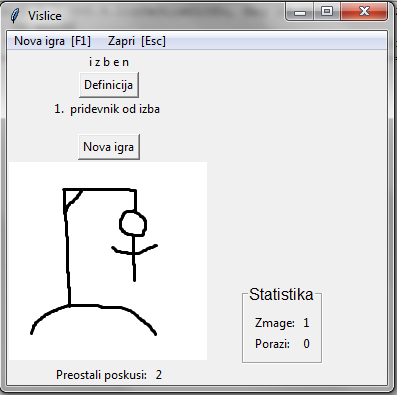
\includegraphics [width=125pt] {slike/za_porocilo_gui_definicija.png}
\caption {Od leve proti desni: grafični vmesnik med potekom igre, ob koncu igre in ob kliku na gumb 'Definicija'.}
\end {figure}

\section {Implementacija in testiranje programa}
Iskanje besed in grafični vmesnik sta bila ustvarjena precej ločeno in združena šele proti koncu. Vsak del je bil sproti testiran, vendar je nekaj napak vseeno ostalo do združitve. \\
Največ težav je bilo pri iskanju definicij, ki se lahko prikažejo na koncu igre, kajti obstaja veliko različnih načinov, kako SSKJ opisuje besede, in potrebno je bilo upoštevati vse. Ker je nemogoče preverjati, ali deluje pravilno za vse besede kar po vrstnem redu, je bila napaka odpravljena, ko je bila opažena pri igri, torej naključno. \\
Za testiranje so bili uporabljeni starši in sošolci. Nekateri njihovi predlogi so bili upoštevani pri spremembi programa.

\section {Zaključek}
Ena izmed prvotnih zamisli je bila, da bi igra poznala več težavnosti in bi izbirala besede, glede na to, kako težke so za uganiti. Zametek tega je viden v neuporabljeni funkcij \textbf {random\_besede}. Vgraditi samo ločevanje težavnosti ne bi bilo težko, saj obstaja že veliko pogojev, ki jim mora beseda zadostiti. Težava nastane pri prepoznavanju, katera beseda je zahtevnejša od druge. \\
Trenutno so vse besede izbrane povsem naključno. Zna se zgoditi, da je izbrana beseda, ki jo vsak pozna in dnevno uporablja. Prav tako je mogoče, da je beseda starinska in narečna. Po eni strani to daje igri težavnost, kajti igralec ne pozna svojega nasprotnika, kot pri običajnih vislicah s prijatelji. Program nima najljubših besed ali črk, po katerih je možno sklepati, kakšno besedo si je izmislil. Igralec lahko samo igra in upa, da bo poznal naslednjo besedo. 
\end {document}